% Infrastructure section 30-01-2011


\input{Sec_SiteInfra/WP1intro}

\input{Sec_SiteInfra/WP1refdef}

\input{Sec_SiteInfra/WP1noise}

\input{Sec_SiteInfra/WP1NN}

\input{Sec_SiteInfra/WP1sitesel}

\input{Sec_SiteInfra/WP1infra}

%\input{Sec_SiteInfra/WP1appendix}

\FloatBarrier
\subsection{Vacuum systems}
%\emph{
%Author(s): C.\ Bradaschia,  G.\ Parguez, A.\ Pasqualetti
%}
\input{Sec_SiteInfra/vacuumparagraph.tex}
\label{WP1vac}
\FloatBarrier
\subsection{Cryogenic service infrastructures}
\label{cryo}
%\emph{Author(s): F.\ Ricci}
We present two possible approaches for the cryo-plants to be set up mainly for the LF- Interferometer.
In fact the HF- interferometer includes just cryo-traps installed at the tube ends for fulfilling  the ultra high vacuum requirements. These traps already present in the LIGO detector and now planned also for  Advanced Virgo,  are based on the use of liquid nitrogen. Similar cryotraps for the ET HF- interferometer have been already presented  in a previous section and from here after  we focus  on the cryogenic requirement of  the LF - interferometer.
The cryo-plant for the LF-interferometer  will provide  the refrigeration power needed to bring the mirror temperature  in the 4 K range. This porpoise can be pursued either by setting up a system based on a battery of cryo-coolers or in alternative using the classic approach of   liquid helium cryostats. In the next we sketch the main characteristics of  ET cryostats. Then we  present and compare the two alternative cryo-plants.


\subsubsection{The ET  cryostats}
%\emph{Author: F.\ Ricci}

In order to reduce the thermal noise impact on the ET sensitivity curve its is sufficient  to cool at cryogenic temperature the four  test masses of the LF- detector. The heat is extracted from the mirror via the suspension fibres attached at the other end to the marionette.  Moreover  the marionette is suspended to the super attenuator which attenuates the seismic noise up to few hertz. Thus,  it is extremely important to preserve the mechanical isolation between the mirror and the cooler system. On the other hand   an efficient  thermal link between
the payload and the cooling system plays is crucial for  the design optimization: we have to 
design  links as short as possible and optimize the  thermal contacts,  in order to avoid 
refrigeration power loss. 
In figure~\ref{fig:cryo_infrastructure_figure/ET_main-cryostat} we report a sketch of the cryo-mechanical system to be adopted for ET-LF.


\begin{figure}[t!]
	\begin{center}
		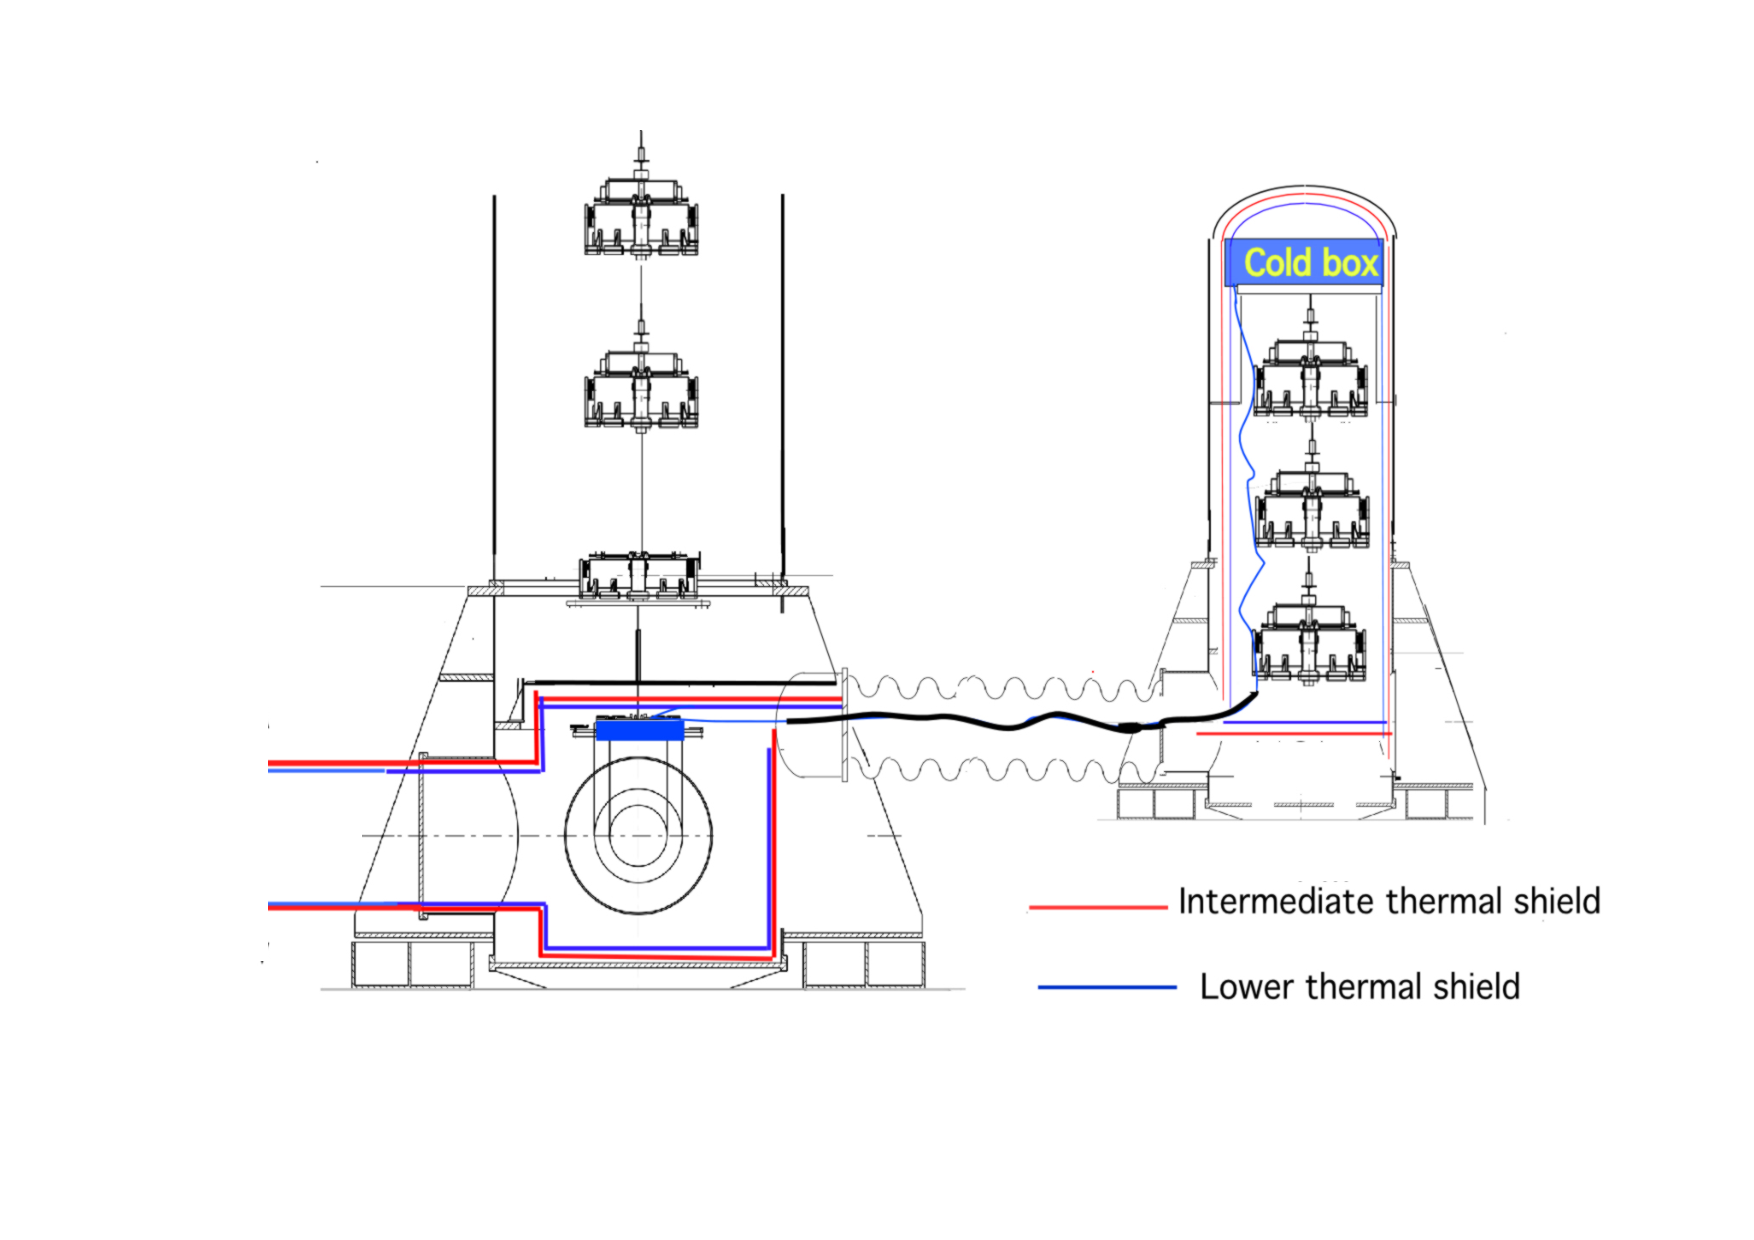
\includegraphics[width=17cm]{./Sec_SiteInfra/Figures/ET_main-cryostat.pdf}
		\caption{Scheme of the cryostats needed for cooling a test-mass of the LF-interferometer.}
		\label{fig:cryo_infrastructure_figure/ET_main-cryostat}
	\end{center}
\end{figure}


The whole payload that we will describe in the suspension chapter is hosted in the lower part of the vacuum tower hosting the 17-m long super-attenuator chain.  The vacuum tower basement is a cryostat  with two thermal screens: the blue line schematizes a surface at $\sim4$\,K, while the red one is the shield at intermediate temperature ($\sim 80$\,K). The upper part and lower part of the tower are separated by a roof  crossed by the Ti-6Al-4V thin rod    which holds the whole payload\footnote{The interface between the upper and lower suspension is described in section~(\ref{Upper_lower_suspension_interface}.}.
The blue line define a volume that has to be vacuum tight. It will permit to cool and warm up faster  the whole payload by  adding pure Helium gas in this experimental volume. Few  mbars of helium   will provide an efficient heat exchange during the cooling phase of the payload from room to cryogenic temperature. Once  the equilibrium temperature is achieved, the helium gas is pumped out before  the laser light injection. 
The basement of the main tower hosting the mirror is connected to an ancillary tower  shown in the figure.
The ancillary tower is  hosting the cold box, which will keep the mirror at cryogenic temperature. The box can be either a simple liquid helium container in the case of a cryoplant based on cryofluids or the cold head of a cryo-refrigerator in the case of a cryocooler plant.

A  thermal line of 20 m maximum length connects the cold box to the last stage of the mirror suspension. It can be made of a  braid  of a high purity material as the electrolytic copper or the grade 6 aluminum (99.9999 \% purity). Both of them  are metals characterized by  thermal conductivity value of 2 kW/m/K in the range 1-10 K. In fact  a braid of   20 m length, made of 8 wires 1 mm diameter can support an heat flow of 200 mW for a temperature  difference  of$\sim$ 1K at the link ends.

To damp the vibration associated  to the cooling system, the soft braid is mechanically coupled to the auxiliary super attenuator chain, hosted in the ancillary tower and   fully complaint with the cryogenic environment. 


In order to define the requirement of  the cryo plant  we have to estimate the cryostat thermal inputs, which depend on the cryostat dimension and the quality of the thermal insulation. 

\noindent
Assuming  that the inner vacuum chamber has to host a mirror with a half meter diameter, we derived the order of magnitude of the thermal input  for the cylindrical cryostats whose dimensions are reported  in the following table:
\begin{table}[htp]
\caption{Cryostat dimensions}
\begin{center}
\begin{tabular}{|c|c|c|}
\hline
\hline
 Container & Diameter [m] & Height [m]\\
\hline
Payload vacuum chamber & 1.5 & 3  \\
Auxiliary tower  & 1 & 2 \\
\hline
\hline
\end{tabular}
\end{center}
\label{tab:cryostat_dimension}
\end{table}

 The thermal super insulation is a standard technique used in the modern cryostats.  The thermal  shield is formed by  highly heat reflective thin layers, set under vacuum  for increasing radiation reflection and decreasing radiation heat transfer through the insulation.  The  most known  implementation   is based on layers  of porous (self-vented) mylar  sheets, which are  aluminized on one side. The sheets are wrapped around the surface to be insulated and  form  a multilayer blanket. 
The mylar is an hydroscopic material incompatible with the HUV requirements of ET. As a consequence the proposed solution implies to  separate the chamber hosting the mirror to the insulation vacuum of the cryostat.   A dedicated pumping system ( rotary-roots-turbo-molecular group) will provide the vacuum insulation.  

Wrapping  25 and 75 layers of self vented aluminized mylar around the two thermal shield, we achieve   the condition to limit the thermal input 
below 1\,W for the 4\,K shields and  around  50\,W for the intermediate ones.
We assume in this evaluation  that the thermal input due to laser light absorbed by the mirror and the thermal radiation emitted by the the km tube is   in the range of few tens of milliwatts  thanks to low silicon absorption at the laser wavelength and to  the helium cryotraps described in~\ref{subsection_helium_cryotraps}. 

It is forth-worth to  evaluate in more details these data in the context of the ET technical design study.  
\FloatBarrier
\subsubsection{The LF-interferometer cryotraps}
\label {subsection_helium_cryotraps}
%\emph{
%Author(s): G.\ Gemme}
\input{Sec_SiteInfra/Cryotraps/cryotraps}

%According the guide lines described above, the overall design of the mirror  suspension and its control system will be very different from those ones presently   used in interferometric antennas. The new system will be the result of a trade off between the need to have a strong thermal contact with the cooling system and the tentative to reduce any dissipation source due to the coupling of the suspension with the mirror.
\FloatBarrier
\etbox{h}{box:information}{The Pulse Tube cryocooler} {The Pulse Tube cryocooler (PT) is based on the displacement and the expansion of a gas, usually helium (He$^4$).  A piston compressor and a rotary valve  are used to create the pressure oscillations ( the typical average pressure in a PT is ${25}$ bar, and the oscillation amplitude is ranging between $2$ and  $7$ bar). Let us refer to the figure \ref{fig:PT_scheme} for explaining the thermal process.
\begin{figure}[H]
	\begin{center}
		\includegraphics[width=9.5cm]{./Sec_SiteInfra/Figures/PT_scheme.pdf}
		\caption{Scheme of a Pulse Tube cryocooler.}
		\label{fig:PT_scheme}
	\end{center}
\end{figure}
We note that  a crucial element of the cryocooler is the  PT regenerator,  a heat exchanger acting as {\it cold storage} systems for the  pulsed flow process.   In practice, the regenerator  stores the energy from one stream and later transfer the energy to a second stream, for example between the out-of-phase pulses of gas. \\
The orifice 1  is connecting  the warm end  to a buffer volume, ten times larger than the volume of the pulse tube so that its pressure is almost constant and close to the average pressure in the pulse tube. The combination of the orifice and the buffer provides a phase difference between the flow of the gas in the tube and the pressure oscillation; such phase difference is necessary for optimizing the PT performance \cite{Mikulin}. The function of the second orifice  is to reduce losses allowing some gas to bypass the regenerator \cite{Zhu} .
\begin{itemize}
\item{When the pressure rises, the gas element moves through the regenerator in the direction of the cold heat exchanger. At the regenerator output  the temperature of the gas element is $T_c$ and enters the tube. There, the gas element is compressed adiabatically, while it moves towards the orifice and  Its temperature rises together with the pressure.}
\item{Now, the orifice 1 is open and  the gas  at pressure $p_h$ flows from the tube to the buffer since  the buffer pressure is lower than that of the tube.}
\item{ The orifice 1 is closed and the rotary valve is set to connect the system to the low-pressure side of the compressor ($p_c$). The gas moves back to the cold heat exchanger and the expansion takes place.  At the end of the expansion step, the pressure of the gas element is equal to $p_c$  and theits temperature is below $T_c$.}
\item{The expansion stops, and the orifice is open again. The gas continues to flow in the direction of  cold heat exchanger and when it is crossing it , the gas warms up to the temperature $T_c$. The amount of heat, which the gas takes away from the heat exchanger, is the cooling power.}
\end{itemize}
To obtain temperatures below 20 K, the system is  operated at low frequency ( $\sim 1$ Hz ).
The frequency defines the diffusion depth $\delta$ in the working gas and the regenerator material:
$$d = \sqrt{\frac {k}{\pi \nu C}}$$
\noindent where $k$ is the heat conductivity, $\nu$ is the frequency and $C$ is the volumetric heat capacity of the regenerator material. Thus, it follows that when the frequency is increased, the diffusion depth decreases, and the heat storage in the regenerator degrades.
Moreover, a high operating frequency leans to a large pressure drop in the regenerator, i.e.\ a poor performance of a system.}
\FloatBarrier
 \subsubsection{The cryogenic infrastructure based on pulse tube cryo-coolers}
 \label{sec:cryocoolers}
%\emph{
%Author: F.\ Ricci}

A simple approach to cool down the mirrors  is based on the use of cryocoolers~\cite{LCGT}. In particular,  
Gifford-McMahon (GM) refrigerators have been developed since a long time and are widely used in various fields of science and industries because of their convenient handling. 
However, their cooling power  is provided by the motion of a displacer which causes large vibrations at the cold head, an aspect which makes them not suitable for all applications where a low acoustic noise level is necessary.

In more recent times,  the pulse tube (PT) cryocoolers  have been developed. 
The particular thermal cycle of PT refrigerators gives them a  two or three  times higher efficiency than GM cryocoolers for loads temperatures between 55 and 120 K, and requires no moving elements at low temperature. This latter characteristic is quite important: because of it, we expect PT refrigerators to be intrinsically more reliable and less noisy than classic GM coolers  \cite{japanoise}. 
Thus, a pulse tube cryocooler seems to be an interesting option for our purposes. However,  because of the gas pulse flowing in its cold head, also this kind of refrigerator injects mechanical noise in the cooled sample, at a level which is still far too high for the elements of a gravitational antenna. Indeed, in order to detect gravitational waves, current detectors have reached displacement 
sensitivities of the order of $10^{-18} m/\sqrt(Hz)$ and an increase by at least two orders of magnitude  is foreseen for ET, where we have to implement the use of low temperatures.

 
 The starting point of the system design is the choice of the pulse tube refrigerator model.
We compared two different models of cryo-coolers, the Cryomech PT 407 and the Sumitomo SRP-052A. For both systems, we measured the acceleration of the $4$ K cold head.

\begin{figure}[t!]
	\begin{center}
		 \includegraphics[width=12cm]{./Sec_SiteInfra/Figures/Sumitomo_Cryomech.pdf}
		\caption{The displacement noise spectrum of the second stage cold point of the CRYOMECH PT407 and of the Sumitomo SRP-052A as function of the frequency.}
		\label{fig:sumitomo_cryomech}
	\end{center}
\end{figure}



Our data show that the vibration noise level generated by the Sumitomo is lower by a factor $\sim 10$ than that by the Cryomech. 
Moreover, our model of Sumitomo has the additional advantage of having the room temperature throttle valve separated from the main body of the refrigerator, with the possibility to keep it far from the cryostat obtaining a further attenuation of the noise produced by this element.
However, the first harmonic generated by the pulse tube is around 1 Hz and it is not attenuated efficiently by the super attenuator chain.  In order to overcome this difficulty, the plan is to apply the technologies developed for  gravitational interferometers and to reduce the vibrations of the cold finger of a PT  cryocooler by an active control system.  In the past we  designed a vibration free cryostat~\cite{VFC}  for limiting the cryocooler vibration, according to the issues discussed above.  The cryostat scheme is sketched in  figure~\ref{fig:cryostat_scheme}.  It is based on the idea to attenuate the cryocooler vibrations by directly acting on it. 
 The cold head vibration  is monitored by  an  optic bundle fibre, a displacement sensor acting as low temperature,  while the actuation is based  on three piezoelectric stacks set  at room temperature outside the cryostat vacuum.  
The cryocooler cold head is clamped to a platform placed on dampers and it is connected to the cryostat by a soft  bellow designed to mechanically decouple it from the cryostat. The feedback correction signal is sent to the three piezo-actuators which are loaded by the platform and can push the cold head platform elastically coupled to cryostat mechanical structure.

\begin{figure}[htbp]
\begin{center}
\includegraphics[width=9cm, height=9.9cm]{./Sec_SiteInfra/Figures/cryostat_scheme.pdf}
\caption{{A simplified scheme of the vibration free cryostat.}}
\label{fig:cryostat_scheme}
\end{center}
\end{figure}


At present the attenuation achieved controlling just the vertical degree of freedom is of the order of $3 \cdot 10^{-3}$.  A further improvement is expected by controlling the horizontal  degrees of freedom and by reducing the recoil effect on the structure holding the monitor sensor of the 4\,K stage. However this active attenuation system is not sufficient and in parallel to this R\&D effort  industrial studies  are under way~\cite{Riabzev} . In particular we cite   the new cryo-cooler  of the AttoCube System \cite{attocube} providing a refrigeration power higher than 1.5 W at 4.2 K  and  very low mechanical vibrations ($< 4.2$ nm peak-to-peak vibration amplitude) measured on a cold  platform decoupled to the pulse-tube cold head.
\noindent
 Moreover new proposals  have been presented \cite{Suzuki_2006}  to reduce the  the cryo-cooler vibration. We discuss  some new ideas in the R\&D section~\ref{cryo_infrastructure_RD}.
 
The  cryo-plants based on PT cryo-coolers implies to install for each tower hosting a test mass a doublet of one stage and two stage PT  cryocoolers. A similar solution is used  to cool the ancillary tower. It will permit to speed up the cooling process  providing  a redundancy during the data taking phase. 
Each PT cold head is driven by a  helium compressor via a couple of high pressure flexible line of a maximum length of 30\,m. 
A larger number of cryocoolers ($\sim 10$) are needed for the helium cryotraps (see~\ref{subsection_helium_cryotraps}).
Each compressor  operates at a pressure $\sim 22$ bar, it requires 5\,l/min of refrigerated water and it absorbs an electrical power drawn at 50\,Hz 
between 5--8\,kW depending on the model. Although they are classified as silent models the typical acoustic noise level at 1\,m distance is $\sim 53$\,dB(A).   
\begin{figure}[htbp]
\begin{center}
\includegraphics[width=12cm, height=8.4cm]{./Sec_SiteInfra/Figures/compressor_mounting.pdf}
\caption{{The standard mounting of a compressor to damp the vibrations.}}
\label{fig:compressor_mounting}
\end{center}
\end{figure}
To reduce the noise trouble, due to the presence of compressors, an underground hall must  be created as a separated part of the main cavern hosting the super attenuator towers.  The wall of this hall has to be treated by a sound insulation system, to avoid noise transmission between the compressor hall and the test mass area (see fig.~\ref{fig:compressor_mounting}). Seen the  number of compressors for each tower and the requested amount   of water flow and electric power  great emphasis must be put on the safety  issues  concerning this auxiliary hall of  $\sim 100\,\mathrm{m^2}$   surface.
We have to notice also that the gas pulse vibration is transmitted also   along  the high pressure helium flexible lines. Thus,  the  line require a specialized design and construction:   it will include  an acoustic sheath covering the flexible tube and massive  concrete slabs to anchor several sectors of the gas lines.


Although this solution has been adopted in LCGT,  we stress that the vibration issue  is one of the  most limiting  factors of a low temperature GW experiment and  it requires a  R\&D activity to be carried on in collaboration with the specialized industries. We conclude noting that recently a new model of cryo-cooler has been developed by the AttoCube System \cite{attocube} providing a refrigeration power higher than 1.5 W at 4.2 K  and  very low mechanical vibrations ($< 4.2$ nm peak-to-peak vibration amplitude) measured on a cold  platform decoupled to the pulse-tube cold head. 



\etbox{r}{box:pro_contra-PT}{Summary of pro and contra of the cryocooler approach}{ 
\begin{table}[H]
\begin{center}
%\caption{Summary of pro and contra of the cryocooler approach}
\color{\contentcolor}
\begin{tabular}{|c|}
\hline
\hline
\hline
{\bf {In favor}} \\
\hline
\hskip 2mm	Higher duty cycle\\
\hskip 2mm	Limited manpower\\
\hline
\hline
{\bf {Against}}	\\
\hline
\hskip 2mm	High level of vibration\\
\hskip 2mm	High electric power consumption in the underground environment\\
\hline
\hline
\hline
{\emph{Infrastructure requirements}}\\
\hline
\hskip 2mm	Distribution of high pressure lines \\
\hskip 2mm	Compressors hosted in auxiliary caverns\\
\hskip 2mm	Efficient water refrigeration system\\
\hline
\hline
\end{tabular}
\end{center}
\label{default}
\end{table}
}
\FloatBarrier
 \subsubsection{The cryogenic fluid approach}
 \label{sec:cryofluids}
% \emph{
%Author: F.\ Ricci}

Cryogenic  fluids in the form of liquid helium and liquid nitrogen are required to circulate for cooling the cryostats of the test masses and the associated cryotraps. 
The heat load requirement at a particular temperature is a prime important factor to select a helium refrigerator/liquefier and to define the dimensions of the nitrogen plant. The cryogenic systems of ET should operate in different modes cool down, steady state and warm up for each test mass tower,
 The cooling time  is a trade off between the need to limit the detector down  time and the  stress due to the thermal gradients 
 During cool down the recommended  flow rate of helium gas will be approximately  $\sim 1$\,g/s. 
 The heat load requirement of cryogenic systems including the transfer loss at steady state is approximately $\sim 20$\,W at 4\,K helium refrigerator/liquefier. A helium refrigerator/liquefier having refrigeration capacity of 160\,W at 4\,K in refrigerator mode and 50\,L/h in liquefier mode without LN2 pre-cooling and 200\,W at 4.5\,K in refrigerator mode and 100\,L/h in liquefier mode with LN2 pre-cooling, is sufficient to guaranty the cooling in the vertex area of the triangular interferometer. In this evaluation a redundancy factor has been included so that  the system will satisfactorily cater the refrigeration load at different state.

 As we anticipated before, to reach a full flexibility of the system, the possibility of performing the cool-down and the regeneration with the main refrigerator has been foreseen too.
The  cryogenic system  will include a distribution valve box and the cryogenic piping up to the interface of the ET cryostat. The distribution valve box contains a 1000 L liquid helium control dewar, a heat exchanger, an electrical heater, a Joule-Thompson cryogenic valve and relevant instrumentation for pressure, temperature and flow rate measurements.
The cryogenic system  has to deliver, in a controlled way, the cooling helium from the refrigerators to the client. It includes mainly a 80\,K gas helium circuit and a 4.5\,K  helium circuit, that can be interconnected through bypass valves; both shut-off valves and control valves are used. The 1000 L liquid helium dewar is used as buffer to stabilize the thermal loads and as re-cooler of the  helium coming from the main refrigerator.  An electrical heater and a cooling system are planned to make the system appropriate to operate an high temperature regeneration (470 K) and to cool it down again to room temperature.

\FloatBarrier
\begin{figure}[htbp]
\begin{center}
\includegraphics[width=14cm, height=8cm]{./Sec_SiteInfra/Figures/He_plant_n.pdf}
\caption{A simplified scheme of the cryogenic plant based on the use of cryofluids.}
\label{fig:He_plant}
\end{center}
\end{figure}


 The redundancy of several elements is added to improve the reliability and the effectiveness of the cryoplant during the experimental conditions and to make it more flexible. 

 The European  industries have demonstrated there ability to construct 
complete  refrigeration systems both  for the needs of the huge accelerator and the associated detectors. 
Thus, the main refrigerators for ET will be realized with proven industrial technologies and tailored on the GW detector needs. It will be  based on Claude cycle and it will provide the coolant helium at the required temperature for cooling the mirror. 
For the liquid helium distribution, we recall here that  long and low thermal loss lines were developed at CERN already in the context of the LEP project. Since this time several improvements in design with respect to earlier lines of similar construction, made it possible to  achieve reproducibly linear heat in-leaks of $\sim 30\,\mathrm{mW/m}$.  At present the  LHC refrigeration system is connected to the 27\,km long accelerator thanks to  high performances helium transfer lines, which exhibit a variety of types, sizes, design choices and layouts. 

In the ET case the refrigerator will be installed on the surface building and the liquid helium has to be sent by  long transfer lines to the underground detector,  like  the case of  the LHC cryoplant. The transfer lines are based on the four-fold coaxial corrugated tube design Each line is made of austenitic stainless steel and the coaxial assembly provides an inner channel  for the supply of liquid or gaseous helium an annular channel acting as a shield for the return of cold vapor, and a common vacuum enclosure for thermal insulation. Low thermal conductivity spacers, made of teflon PTFE are set between the outer tube, return channel and supply pipe. The outer corrugated tube of the return channel is also super-insulated by several layer of aluminized mylar (see figure~\ref{fig:transfer_line}).

\FloatBarrier
\begin{figure}[htbp]
\begin{center}
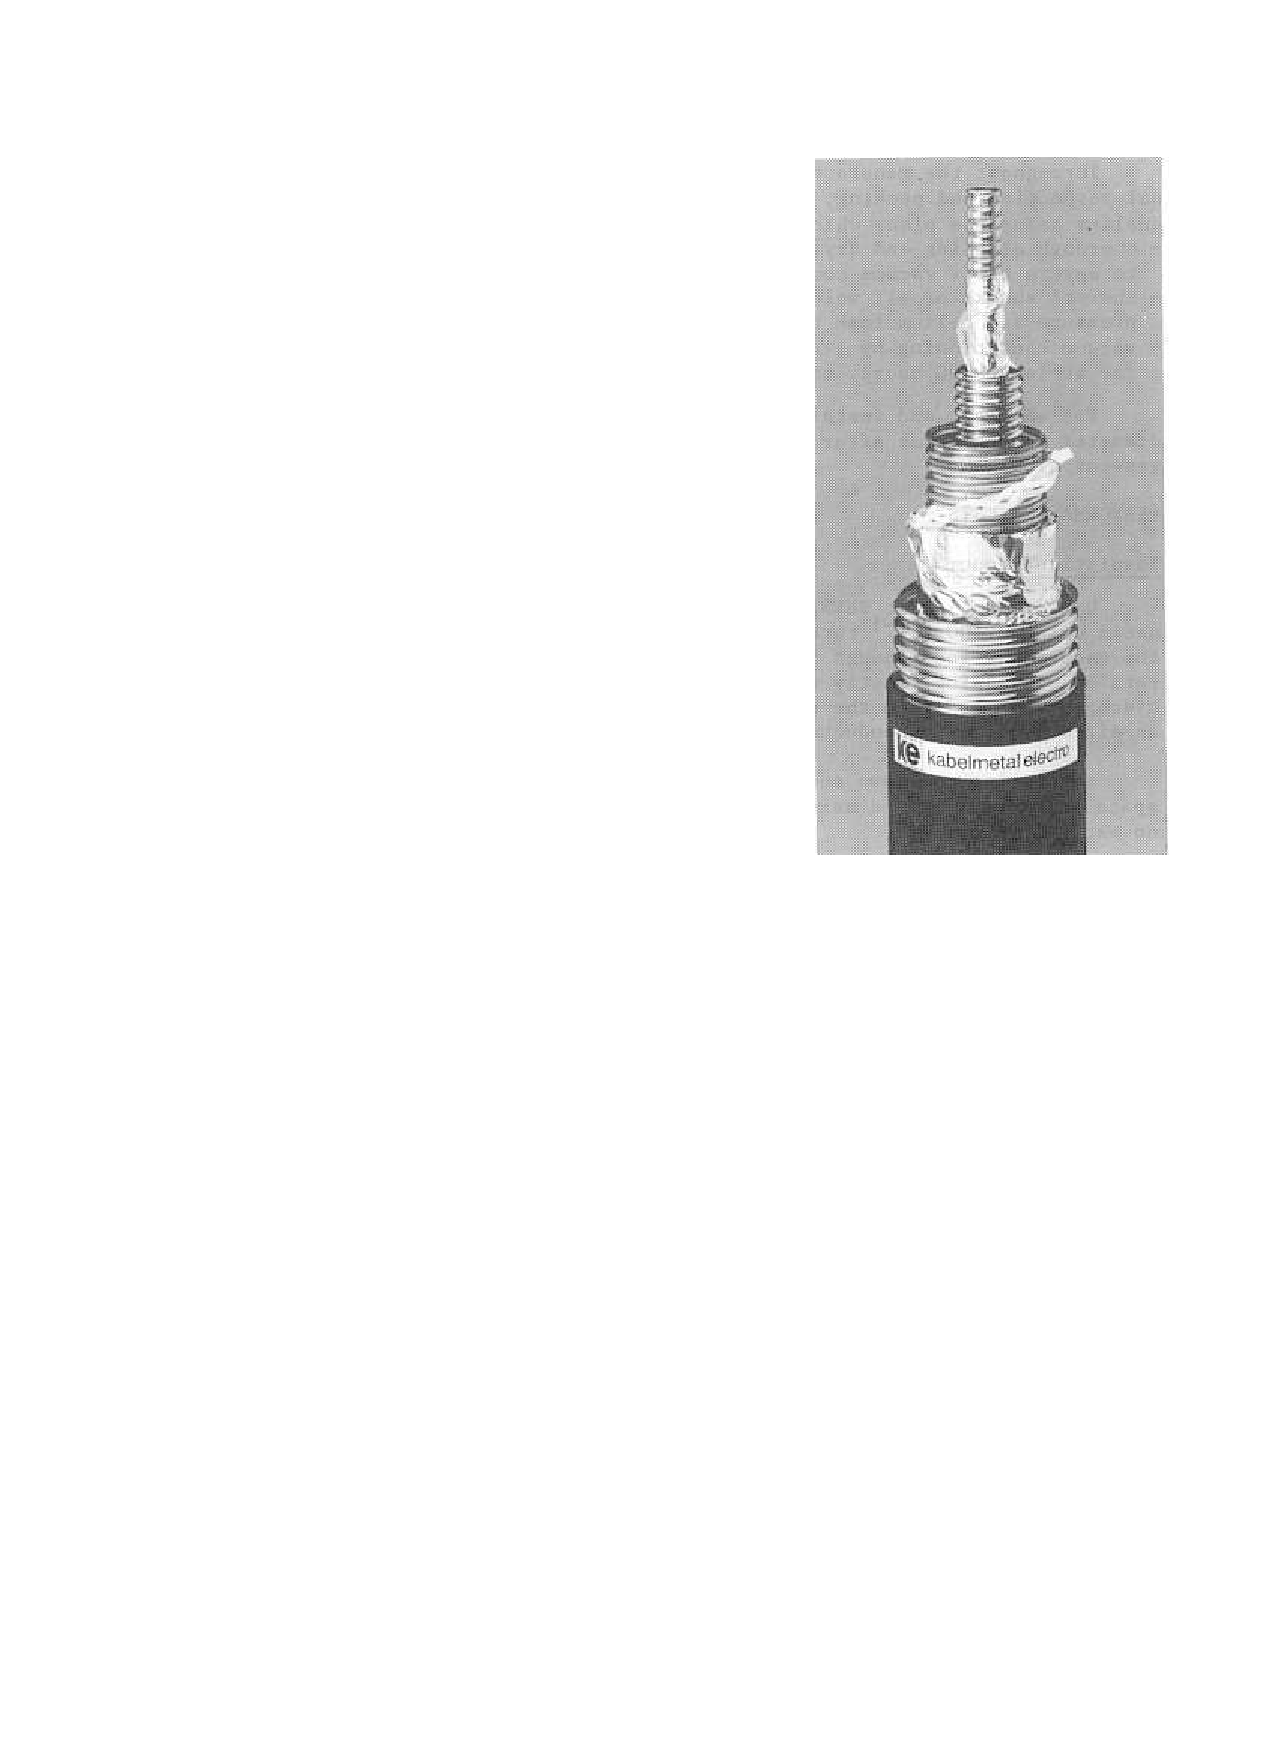
\includegraphics[width=5cm, height=7cm]{./Sec_SiteInfra/Figures/transfer_line.pdf}
\caption{A cross section of a flexible transfer line developed at CERN in collaboration with Kabel Metalelectro~\cite{Lebrun}}
\label{fig:transfer_line}
\end{center}
\end{figure}


In order to reduce the quantity of impurities in the helium and to recover the gas, a  Purification and Recovery System is implemented in the cryogenic plant. It is composed by a helium vaporizer, a high pressure recovery compressor and a helium cryogenic purifier system. An atmospheric gas bag (100 $m^3$), high pressure containers (20 bottles at 20 MPa, 10 N m$^3$ each) for impure gas helium, 3 medium pressure tanks (30 $m^3$ at 2 MPa) for pure gas helium, a liquid nitrogen container (50,000 L) and dedicated transfer stainless steel pipe lines are provided for the fluids storage. The helium to be recovered is collected in the gas bag; if its temperature is too low to enter in the gas bag, the cold helium is sent to a vaporizer where it is heated to the ambient temperature before entering the helium gas bag. The helium coming from the gas bag is sent to the recovery compressor and stored in the high pressure (20 MPa) bottles from which is delivered to the impure gas storage. The impure gas helium flows to the purifier and then it is stored in medium pressure (up to 2 MPa) pure helium buffers connected to the cycle compressors.





The cryoplant will be installed in a building close to the main experiment building on surface. To reduce the noise trouble, due to the presence of compressors, a cryogenics compressor hall will be created as a separated part of the technical supplies building. The wall of this hall will be treated by a sound insulation system, to avoid noise transmission between the compressor hall and the other building. 



\FloatBarrier

\subsubsection{Cryogenic plant control}
\label{sec:cryo_comtrol}
%\emph{
%Author: F.\ Ricci}

The cryoplant design and the technical solutions to be adopted are focused on the optimization of  the system performances and it will be conceived  to implement all the required operative scenarios in a fully automatic mode.

The facility control system, based on a master/slave architecture,   will be split into three plants (each for interferometer vertex ) and three distinct supervisory systems will be  provided with engineer and operator workstations. The three control systems will be  independent, but inter communication signals will be exchanged among the station units.
The internal structure of the cryogenic control system will be based on PLCs (Programmable Logic Controllers), equipment of proven reliability in the industrial environment. A PLC will act as master of the local unit PLCs, with the purpose to coordinate the cryoplant activities and interface the logic unit with the upper subsystem level. Feedback control will be necessary to control for example the speed of the turbines or other parameters like temperature and pressure of the helium in different part of the cryogenic system; since the time constraints are not strict (response times of the order of seconds), the control routines will be executed without problems by PID (Proportional-Integral-Derivative) controllers inside the PLCs. A commercial off-the-shelf Supervisory Control and Data Acquisition system will be employed to monitor the plants, for operator intervention, commissioning, test purposes and data storage.


\FloatBarrier
 \subsubsection{A  future development: lowering the temperature  with Helium II}
\label{sec:Helium_II}
%\emph{
%Author:F. Ricci}

In order to increase the cooling efficiency and to get a further reduction of the thermal noise contribution, in the ET future we can plan to cool down to the $\lambda$ point  the thermal bath used for cooling the mirror.   In principle the use of the liquid helium II (He II) has great advantages: it limits the vibration noise associated to the other cryogenic fluids \cite{lambda} and it provides a powerful way  for extracting the heat  from the mirrors.
 Modern large engineering projects for high-energy physics require thermostatic control of working components at the level of $1.8$ -  $2$ K and are constructed  with lengths of channels containing He II. The uniqueness of He II is that it contains a superfluid component with zero entropy, which moves through other liquids and solids with zero friction to an extent dependent on the temperature of the liquid.
  He II is a liquid of extremely low viscosity and very high heat capacity, which prevents  small transient temperature fluctuations. Moreover, thanks to its very high thermal conductivity is able to conduct away heat a thousand times better than any metallic conductor like copper.

     In He~II, the heat from a hot surface is carried away by the superfluid component, so in any design with complicated geometry and  helium flows, the entire heat load acts on the phase interface. The boiling mechanism 
involves evaporation from surfaces ad in a flow of ordinary boiling liquid, the heat influx is uniformly distributed in unit volume of the two-phase mixture. In stratified He~II, the heat influx is associated with the interface between the phases, so the He~II evaporation rate is increased by a substantial factor. 
A major feature of boiling in He~II is that the evaporation of the superfluid component predominates. The heat load 
is transported by convection in the superfluid component, and this consequently evaporates more rapidly than does the normal component. 


When a two-phase flow of He~II moves in a heated channel, a droplet structure or mist is formed in the vapor space as the amount of liquid in the stratified flow decreases. In a stratified flow of an ordinary liquid in a large-diameter tube, an increase in the bulk vapor content  leads to the vapor becoming superheated and the liquid evaporating completely. 
In He~II one prevents the vapor becoming superheated  by encouraging the spontaneous formation of a droplet structure with a large heat-transfer surface, which provides a constant temperature over the channel cross section. 


An efficient and quiet configuration for cooling the mirror by He~II is the {\it bain de Claudet}. Here the idea is to provide  superfluid helium at atmospheric pressure and to insure continuous refilling from the container of the helium in the normal state. In this way the He~II bath is kept  in a quiet hydrodynamic status well far from the boiling point .
In this case the cold box on top of the super attenuator of the ancillary tower  is an  heat exchanger   filled by superfluid helium at atmospheric pressure and operating in the stationary condition of zero mass flow, which  implies $\rho_s v_s = - \rho_n v_n $ in absence of the vapor phase, where $\rho$ and $v$ are the density and the velocity of the normal $(n)$ and superfluid $(s)$ components\cite{ricci}. 
 

  The He~II mirror  cooling approach  requires also a deeper analysis of the  impact of  the acoustic losses of the fluid to the dynamic behavior of the suspended  test masses. 
This effect should depend  on the hydrodynamic regime of the  helium II. In particular  we need to consider the interaction mechanism between the two liquids (normal and superfluid), which determines the heat transport. In the case of a superfluid helium vortex formation this is  described by the Gorter-Mellink  force per unit length, which results  a function of the velocity  difference $\vert \vec v_n - \vec v_s \vert$. For a one dimensional helium flow $f$ can be written as  

\begin{equation}
f = {\frac{\rho_n \rho_s}{({\rho_ +\rho_s})^2}} \eta_n \vert \vec v_n - \vec v_s \vert
\label{eq:Gorter_Mellink}
\end{equation}  
\noindent
where $\eta_n$ the viscosity of the normal fluid. 

Moreover   the design of the heat exchanger providing a sufficient refrigeration power is not straightforward. In fact the velocity difference of the two fluids depends  strongly  on the geometry of the heat exchanger, the nature of the material in contact with the fluid  and the status of the contact surfaces. In conclusion in order to  assess  the validity of the cooling approach for the cryogenic design of the ET detector, we need  to develop a complete hydrodynamic model including   vapor phase and  extra interaction terms as well as a deep R\& D activity and prototyping.


\FloatBarrier
\subsubsection{R\&D in Cryo-coolers}
\label{cryo_infrastructure_RD}
%\emph{
%Author: F.\ Ricci}

As we pointed out in the previous section the focus of the R\&D activity for cryo-cooler will be on the reduction of the vibration generated by the pulse tube.
The pulsed force due to the gas deforms the tube of the cold head displacing the cold plate of several microns. These effect has been simulated via finite element software showing that in function of the the cold geometry the longitudinal expansion of the tube can be of the same order the horizontal displacement.  Thus, there is a large margin of improvement on the active attenuation damping of the harmonics associated to the gas pulse.  

Moreover  it has been proposed to modify the mechanical design of the cold head to  reduce the displacement vibration. Several attempt have been done already by several groups in the world, using different tube material, adding glass fibre support or using coaxial geometry~\cite{Koettig}.

An interesting idea has been proposed by Suzuki  to utilize the vibration as counter force to compensate the pulse tube expansion with the constraint to adopt a compact configuration. In practice adding to the same cold head  a couple of tubes  pressurized by a  gas wave with opposite  phase  to the other couples we can obtained a cancellation effect.
In figure~\ref{fig:Suzuki} we show a first test carried on at KeK they tied improved  the cancellation  by adding more than one couple of tubes with suitable phase difference. 

\begin{figure}[htbp]
\begin{center}
\includegraphics[width=5.4cm, height=4cm] {./Sec_SiteInfra/Figures/Suzuki.pdf}
\caption{The pulse tube scheme proposed and tested by T.~Suzuki at Kek~\cite{Suzuki_2006}}
\label{fig:Suzuki}
\end{center}
\end{figure}



As we discussed in the previous section~\ref{sec:Helium_II}, there are significant advantages to lower the temperature below the $\lambda$ point and we can succeed to lower the temperature by modifying  the cryoplant based on cryogenic liquids. However, the same temperature can be achieved using cryo-coolers.  The standard two-stage PT  operate with ${}^4$He as working fluid. Consequently the minimum no-load temperature of these PTs was above 2\,K, because the thermodynamic properties of ${}^4$He near the superfluid phase transition prevent cooling to lower temperatures. A regenerative cryocooler can cool below 2\,K when ${}^3$He is used as working fluid instead of ${}^4$He. This approach was pursued and  a minimum stationary temperature of 1.27\,K  was achieved and  at 4.2\,K  the cooling power  was found to be larger than with ${}^4$He~\cite{Thummes}. This result has to be regarded as the starting point of a possible evolution of the ET cryo-cooler plants, which requires higher refrigeration power and less vibration.
 To succeed in getting a significant improvement without spoiling the refrigerator performance a strong interaction with the PT experts and specialized cryogenic industry has to e set up.



% \bibitem{Lebrun} H. Blessing, Ph. Lebrun, K. Schippl " Very low-loss liquid helium transfer with long fexible cryogenic lines" , CERN LEP-MA/89-38



% \bibitem{vanSciver}
% S. W. Van Sciver, Helium Cryogenics, Plenum Press, New York (1986)

% \bibitem{Kapitza}
% P. L. Kapitza, The study of heat transfer on Helium II, J. Physics (USSR) 4, 181(1941)

% \bibitem{Khalatnikov}
% I. M. Khalatnikov,  Introduction to the theory of superfluidity, Chap III, W. A. Benjamin, New York, (1965)

% \bibitem{Koettig}
% T. Koettig , F. Richter , C. Schwartz , R. Nawrodt , M. Th�rk and P. Seidel , Cryocooler 15 � Int. Cryocool. Conf. Inc. , Boulder


% \bibitem{Xu}
% M.Y. Xu , A.T.A.M. De Waele, Y.L. Ju, Cryogenics 39, 865 (1999) 

% \bibitem{Thummes}
% N. Jiang, U. Lindemann, F. Giebeler, and G. Thummes, Cryogenics 44,  809 (2004) 

% \bibitem{Qiu}
% Limin Qui, YonglinHe, Zhihua Gan, Laihong Wan, Guobang Chen , Chinese Science Bulletin, 50, 1030 (2005)




% \end{thebibliography}







%\FloatBarrier
%\subsection{Safety Issues}
%Safety and health would have the highest priority in the engineering of a deep underground laboratory and would be fully integrated into the design of laboratory activities at every stage of planning, design and construction. An underground laboratory would also provide an ideal laboratory for research and development leading to advances in underground safety systems and technology. Scientists and engineers could carry out safety and health research within a deep, controlled underground setting. Particular attention would go to advances in key areas such as underground communication, ventilation, access, emergency egress and refuge design. During all phases of operation (e.g.\ from construction to science operation) safety policies and guideline will have to be in place with regards to: 
%\begin{itemize}
%\item{Construction of the ET infrastructure:}
%During the construction of the ET infrastructure the safety of both engineering and scientific personnel has to be insured. Hazards at this phase include explosions, strata collapse, vehicle collisions, fires, inundation, drowning and asphyxiation.    
%\item{Commissioning and scientific operation:}
%During this phase it is assumed that construction has been completed. Hazards that have to be addressed are: strata collapse, explosions, water inundation and drowning, electrocution, fire, cryogens (e.g.\ rapid expansion > asphyxiation), and chemicals like sulphide minerals etc.
%\item{Escape routes and fire doors: compartmentalising}
%\item{Cost examples from other underground facilities}
%\end{itemize}



%\FloatBarrier
%\subsection{Computing infrastructures}
%\emph{
%Author(s): T.\ Dent, S.\ Aoudia
%}
%\dots


\input{Sec_SiteInfra/WP1cost}


%\FloatBarrier
%\subsection{Cost estimate}
%
%Preliminary cost analyses have been performed in order to optimize the cost-to-performance ratio
%for the ET Reference Design. Various components costs were estimated, options compared and
%significant cost-driven changes were implemented will maintaining the scientific performance goals.
%The estimates were based on numerous European-wide tenders and using the lowest
%reasonable price for the dedicated specifications. In addition, estimates were made of the
%explicit work force needed to support the respective activity. Four classes of cost are
%distinguished
%\begin{itemize}
%	\item{} Site specific costs
%	\item{} Infrastructure costs
%	\item{} Detector costs
%	\item{} Operating costs
%\end{itemize}
%
%The total estimated value for the ET Reference Design is xx MEuro (in 2010 \euro). 
%An important result of the value costing is that it provides a basis for
%determining the relative value of various components and work packages. This
%enables an equitable division of commitments of the partners in the ET consortium.
%
%The site specific costs for the ET Reference Design are related to the direct costs
%for providing the infrastructure to site the observatory and are estimated at xx MEuro
%(2010 value level). These costs include the underground civil facilities, services
%(electricity and water distribution), buildings and surface construction. These costs
%are site dependent and have been considered for a range of European sites. It
%should be noted that the actual site-specific costs will depend on the location
%where the observatory is constructed, and the facilities that already exist
%at that location.
%
%The infrastructure costs include the direct costs for the
%safety and security systems, the vacuum system and the cryogenic infrastructure.
%
%The explicit labor required to realize the construction project is estimated at
%xx million person-hours. It includes administration and project management,
%installation and testing. Part of the labor will be contracted and part will come from
%existing labor in collaborating institutions.
%
%\begin{figure}[htbp!]
%	\begin{center}
%		\includegraphics[width=10cm]{./Sec_SiteInfra/Figures/ETcost1.pdf}
%		\caption{Cost breakdown of the ET Reference Design in single interferometer mode.}
%		\label{fig:etcost1}
%	\end{center}
%\end{figure}
%The cost breakdown of the ET Reference Design in single interferometer mode
%is shown in Fig.~\ref{fig:etcost1}. This configuration constitutes the phase I instrumentation
%of ET and features a single xylophone interferometer. Phase II will be realized later
%and features a triple xylophone interferometer configuration.
%
%The figure shows that the main cost drivers are the underground site infrastructure
%and the vacuum system. A breakdown of these main cost components is given
%in Figs.~\ref{fig:etcost2} and \ref{fig:etcost3}.
%\begin{figure}[htbp!]
%	\begin{center}
%		\includegraphics[width=10cm]{./Sec_SiteInfra/Figures/ETcost2.pdf}
%		\caption{Partitioning of the site specific costs of the ET Reference Design.}
%		\label{fig:etcost2}
%	\end{center}
%\end{figure}
%Fig.~\ref{fig:site} shows that the main cost drivers are the tunnels and caverns.
%Note that the cost of tunneling is site dependent. For the estimates we have
%used $260\,\euro / \mathrm{m^3}$ for the excavation costs. Several underground sites in Europe
%have been identified that comply with such costs, although a significant
%bandwidth applies. The number is also compliant with the site costs for
%LCGT in Japan.
%
%\begin{figure}[htbp!]
%	\begin{center}
%		\includegraphics[width=10cm]{./Sec_SiteInfra/Figures/ETcost3.pdf}
%		\caption{Partitioning of the costs for the vacuum system of the ET Reference Design.}
%		\label{fig:etcost3}
%	\end{center}
%\end{figure}
%The vacuum vessel constitutes the main cost driver for the vacuum system.
%In addition, the bake-out equipment is a significant cost driver. In order to
%realize the vacuum system at the estimated cost, it will be needed to set-up
%3 vessel construction facilities at the ET site. 
%
%The budget estimate is structured as follows. 
%\begin{enumerate}
%\item{} Facilities
%\begin{enumerate}
%\item{} Manufacturing facilities
%\begin{enumerate}
%\item{} Factories: vacuum tube construction
%\item{} Shops: mechanical, electronics workshops
%\item{} Preassembly: cleanroom facilities
%\item{} Testing
%\end{enumerate}
%\item{} Conventional facilities
%\begin{enumerate}
%\item{} Sites: main site and two satellite sites
%\item{} Buildings
%\item{} Tunnels
%\item{} Caverns
%\item{} Main shafts
%\item{} Midway shafts
%\item{} Utilities
%\item{} Environmentals
%\end{enumerate}
%\end{enumerate}
%\end{enumerate}
%
%Estimates for the cost of Einstein Telescope Reference
%Design in single interferometer mode (phase 1) are given in Table 1.1.
%
%
%
%\medskip
%\noindent
%{\bf Project table 1.1.} {\sl Budget estimate for the Einstein Telescope Reference
%Design in single interferometer mode (phase 1).}
%
%\medskip
%\begin{center}
%\begin{tabular}{|l||r|}\hline
%Subsystem & Cost \\
% & [ Euro ] \\ \hline
%Site and infrastructure & 10,000 \\
%Buildings &  10,000 \\
%Safety system & 10,000 \\
%Vacuum system & 10,000 \\
%Cryogenics & 10,000 \\
%Optics & 10,000 \\
%Suspensions & 10,000 \\
%Geophysics & 10,000 \\
%Control system & 10,000 \\
%Computing & 10,000 \\
%& \\
%{\bf Total} & {\bf 10,000 PlEuro}\\ \hline
%\hline
%\end{tabular}
%\end{center}
%
%Site requirements that impact construction cost must be considered. These include topography and geological 
%subterranean conditions. Factors such as horizontal VS vertical access to the underground facilities greatly 
%affect the construction costs. Site availability and acquisition cost can vary greatly. Availability of existing 
%support infrastructure is important. Underground laboratories as Laboratorio Nazionali del Gran Sasso LNGS 
%(Italy), Laboratoire Souterrain de Mondane LSM (France), Laboratorio Subterraneo de Canfranc LSC (Spain) 
%and Institute for Underground Science, Boulby mine (UK) provide extensive facilities for scientific and technical 
%staff. This includes accommodations for resident staff (housing, schools, etc.), and visiting staff (lodging, 
%transportation, etc.). For the same reason active or closed down mines may provide valuable facilities such 
%as hosting shafts, electrical infrastructure, water pumps, and safety systems. In addition, they may provide 
%local technical support and experienced technical staff. Other factors that determine the (cost of ) the main 
%infrastructure design include groundwater conditions, hydrology and drainage which have an impact on the 
%design of buildings and tunnels, accessibilities such as roads, railroad, distance to nearby supporting technical 
%facilities, site utilities installations as power, water, and sewage. Finally, labour cost and proximity of soil waste 
%and borrow areas must be considered. 
%
%Aside from construction costs, there are various factors impart the operation cost. These include the cost of
%electrical power, cost of local labour, heating and cooling requirements, maintenance, and travel time and 
%cost for visiting staff. Environmental, health and safety plans must be put in place to assure the safety of
%users, staff and visitors to ET. These plans must comply with the relevant governmental and European
%standards and regulations. It is important to elevate the life-safety level above that in the mining and
%underground construction industries to one appropriate for researchers, students, and the public. 
%
%Risk must be minimized in the realization of ET. Risk factors include acquisition risk, risk from environmental 
%sources such as earthquakes, floods and storms. Special attention must be paid to potential future man-made 
%noise and vibration from development or industrial projects. 
%\FloatBarrier
%\subsection{Technologies to be developed}
\input{Sec_SiteInfra/WP1randd}



